
\subsection{Benchmarks}

\begin{figure}
\centering
   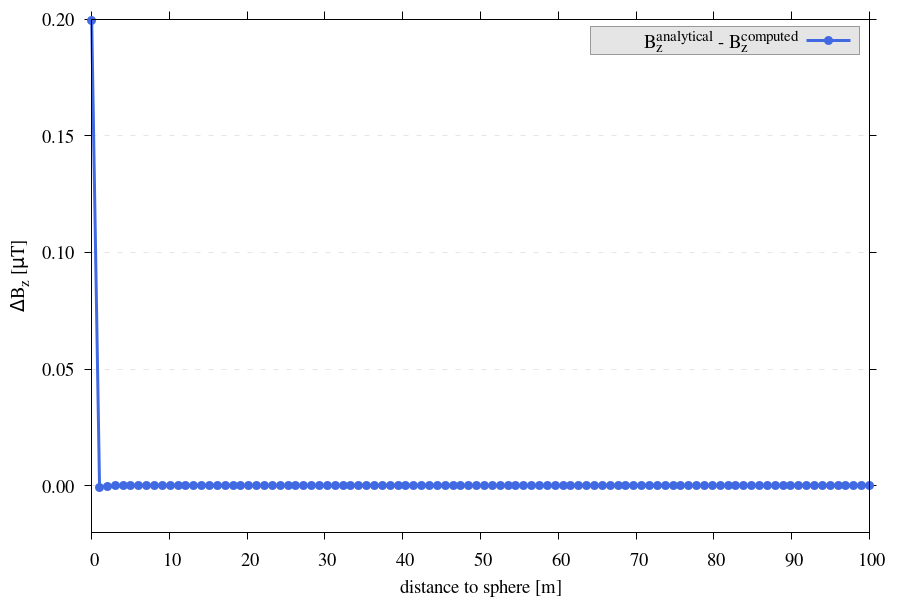
\includegraphics[width=1\columnwidth]{Afbeeldingen2/Benchmarks/B1dipole_dif.png}
    \caption{Difference between analytical solution for a single dipole and computed values at increasing distance from surface of a sphere. }
    \label{fig:dipoleresults}
\end{figure} 
\subsubsection{A single dipole}
Equation \ref{eq:singledipole} provides us with a solution for the magnetic field produced by a single dipole \parencite{GRIFFITHS,BLAKELY}. At very large distances, a sphere of uniform magnetization can be seen as a single dipole of volume $V=\frac{4}{3}\pi r^3$, where $r$ is the distance from $\mathbf{P}$ to the center of the sphere $z-z_s$ \parencite{BLAKELY}. If we align the magnetization of the sphere with one of the axes, $\mathbf{M}=(0,0,M_{z0})$ and compute values on a line above the center of the sphere, $\mathbf{r}=(0,0,z-z_s), r=z-z_s$,  eq.  \ref{eq:singledipole} reduces to
\begin{equation}
\mathbf{B}_{dip}(\mathbf{r}) = \frac{\mu_0 V}{2\pi} \frac{M_{z0}}{r^3}   \mathbf{e}_z
\end{equation}
The model setup was as follows: A spherical inclusion of radius $ds=1m$ and $\mathbf{M}= (0,0,7.5) $ in a domain of 2x2x2m with a resolution of 100 elements in each direction. The magnetic field values were computed along a vertical line positioned directly above the sphere's center, where the distance $r$ was progressively increased to exceed 1000m.  As illustrated in Figure \ref{fig:dipoleresults}, the discrepancies between the analytical solution and computed values are minimal. Even at a height of  $0.25$m, the smallest height above the topography measured in the Etna case study \parencite{Meyer23}, the error remains approximately $\sim|0.01| \micro T$ . 

\subsubsection{Internal cancellation}
According to theory, all internal magnetic forces, or contributions, on the surfaces within the magnetized object should cancel out \parencite{JACKSON}. Hence, regardless of variations on the internal surfaces of elements in our domain, the computed values at any point above the surface should be consistent. To verify this, a domain of 10x10x10m, with an initial element size of 2x2x2m and $\mathbf{M}= (0,1,0)$, was deformed in two ways: \\ (1) a random value between $-0.1$ and $1$ was added to the z coordinates of internal nodes \\ (2) situation in (1) was combined with elements of a very high aspect ratio (5x1x0.2m). As expected, the computed values of the magnetic field on the observation plane, located one meter above the domain, remained consistent (up to machine precision) across these scenarios. 

\subsubsection{A magnetized sphere}
Using the boundary conditions of a magnetized ($M$) sphere present in a magnetic field $\mathbf{B_0}$, equation \ref{eq:Bsumfinal} can be rewritten to equation \ref{eq:Bsumsphere} (for derivation see appendix \ref{app1}). This is applicable if the sphere is uniformly magnetized with $\mathbf{M}$ parallel to $\hat{k}$, the polar direction and if the origin of the coordinate system is placed at the center of the sphere (see Figure \ref{fig:sphere}). Then, the magnetic field outside this sphere is defined as \parencite{REITZ}
\begin{equation}
    \label{eq:Bsumsphere}
    \mathbf{B_t(r)} =  B_0\mathbf{\hat{k}} + \frac{\mu_{0}}{3}M\left(\frac{a^3}{r^3}\right) \left(2\mathbf{\hat{r}}\cos{\theta}+\mathbf{{\hat{\theta}}}\sin{\theta}\right)
\end{equation}
where $r$ is the distance from the center of the sphere to the observation point, $a$ is the radius of the sphere, $\mathbf{\hat{r}}$ is the unit vector in the direction of $r$, $\mathbf{\hat{\theta}}$ is the unit vector in the direction of $\theta$, $\theta$ is the angle between $\mathbf{\hat{r}}$ and $\mathbf{\hat{k}}$ increasing clockwise from $\mathbf{\hat{k}}$ and both $\mathbf{M}$ and $\mathbf{B_0}$ are in the direction of $\mathbf{\hat{k}}$. See Figure \ref{fig:sphere} in appendix \ref{app1}. for visualisation.
\begin{figure}
  \centering
        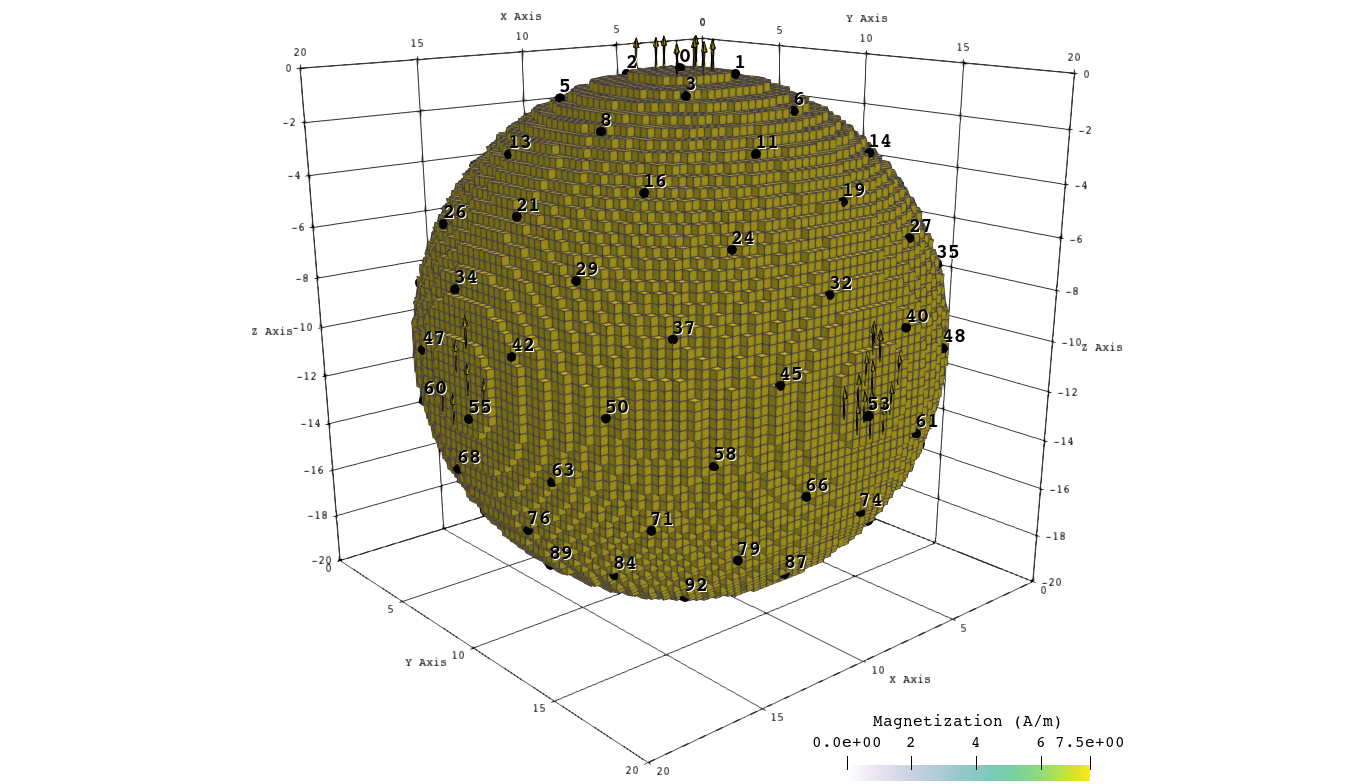
\includegraphics[width=0.4\linewidth]{Afbeeldingen2/Benchmarks/Model setup_numbering_framed_larger.png}
    \caption{Visualization of the model setup, numbering along Fibonacci spiral for uniform distribution above the tessellated sphere.}
  \label{fig:sphere_bench_setup}
\end{figure}
The model setup was as follows: A spherical inclusion similar to the first benchmark, but now with a radius of $a=$ 10m was placed in a domain of 20x20x20m and $\mathbf{M}= (0,0,7.5)$. Since a sphere is a complex shape to accurately represent using hexahedron elements, a large number of elements were anticipated to be necessary to produce adequate results. A Fibonacci spiral was used to uniformly distribute 100 computation points at 0.25m and 0.5m above the surface of a sphere with a resolution of either 3 el/m or 6 el/m. The results are shown in the Figure \ref{fig:sphere_bench}. As expected, closer to the surface the required resolution increases, however, at distances $\sim 0.5$m above the sphere 3 el/m suffices. 

\begin{figure}
\centering
   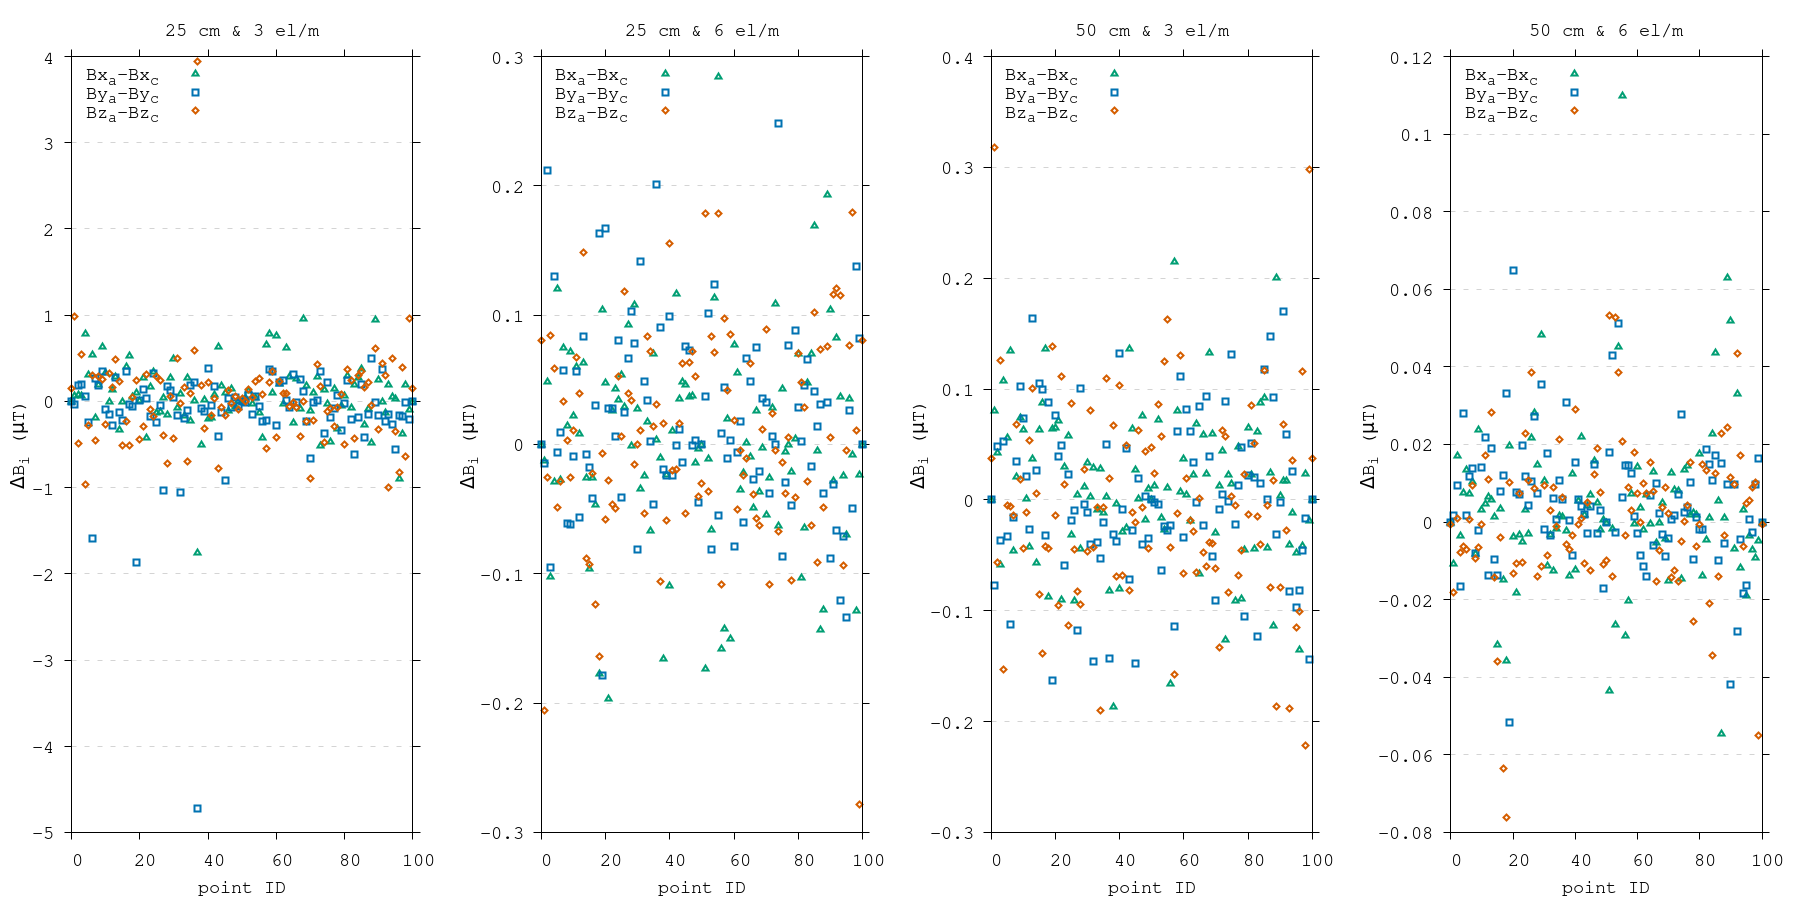
\includegraphics[width=1\columnwidth]{Afbeeldingen2/Benchmarks/B3sphere_dif_mp_splitcase_all.png}
    \caption{Difference between analytical solution and computed values for 100 difference computation points at either 0.25 or 0.5m above the surface of a sphere with a resolution of either 3 or 6 el/m. Numbering of the computation points start at the top of the sphere and circle down in a counterclockwise fashion.  }
    \label{fig:sphere_bench}
\end{figure} 

\begin{figure}
\centering
   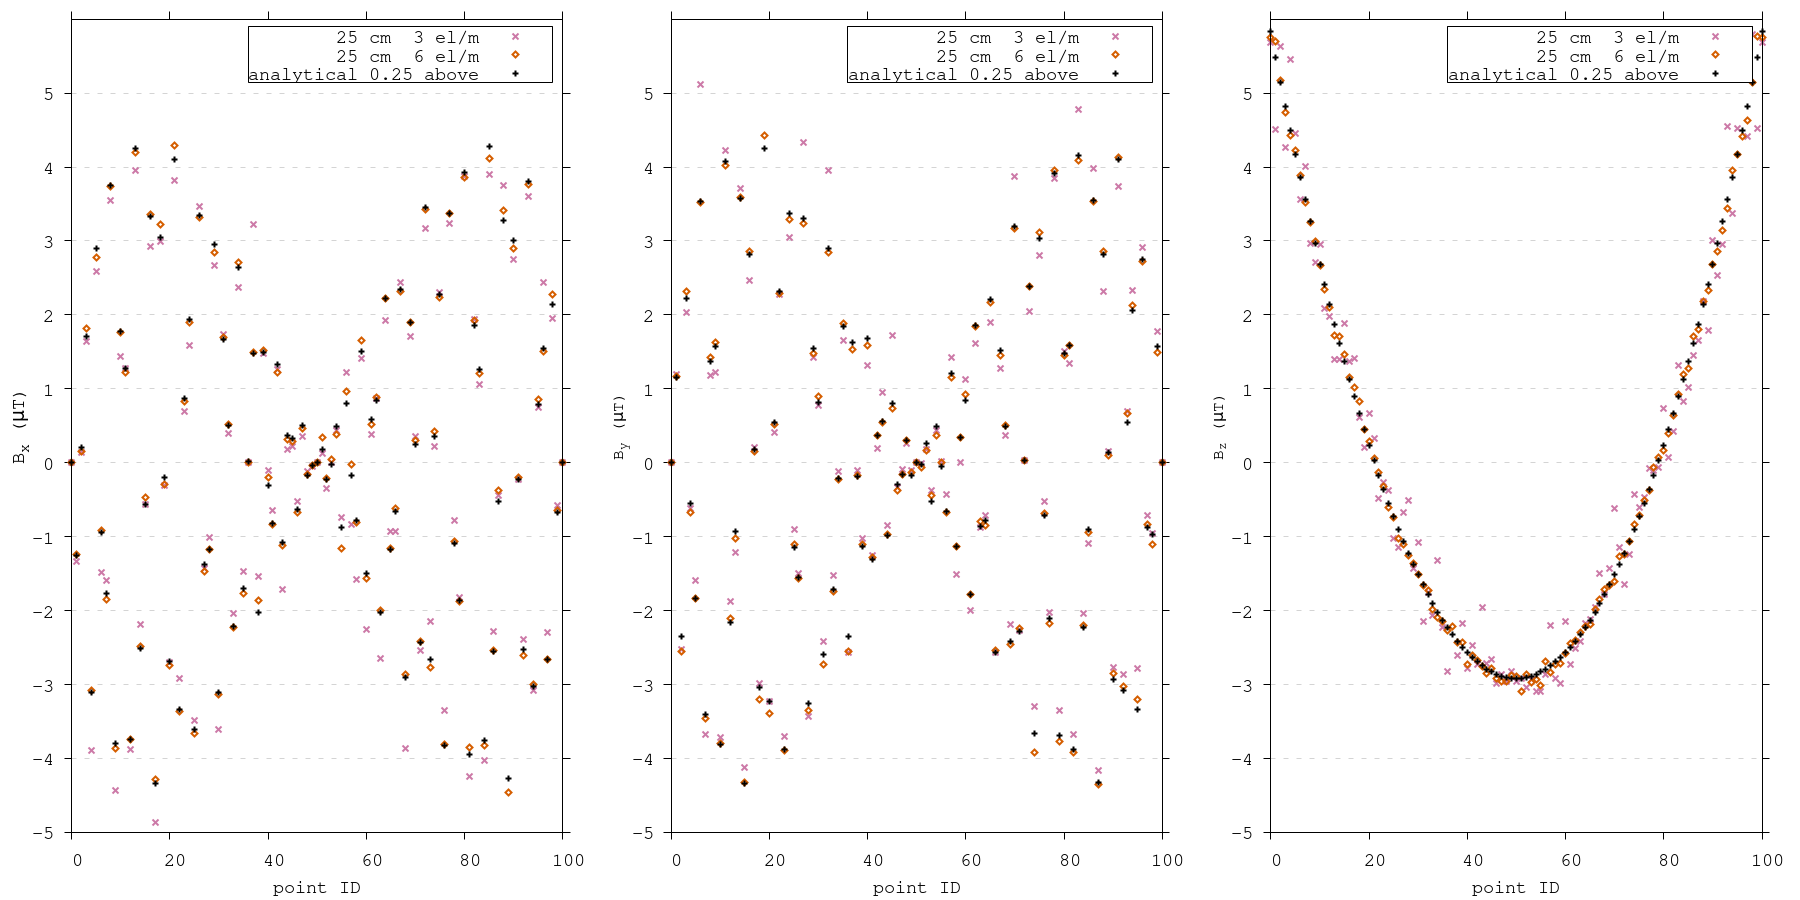
\includegraphics[width=1\columnwidth]{Afbeeldingen2/Benchmarks/B3sphere_mp_025.png}
    \caption{Difference between analytical solution and computed values for 100 difference computation points at either 0.25 or 0.5m above the surface of a sphere with a resolution of either 3 or 6 el/m.  Numbering of the computation points start at the top of the sphere and circle down in a counterclockwise fashion.  }
    \label{fig:sphere_bench}
\end{figure} 
\begin{figure}
\centering
   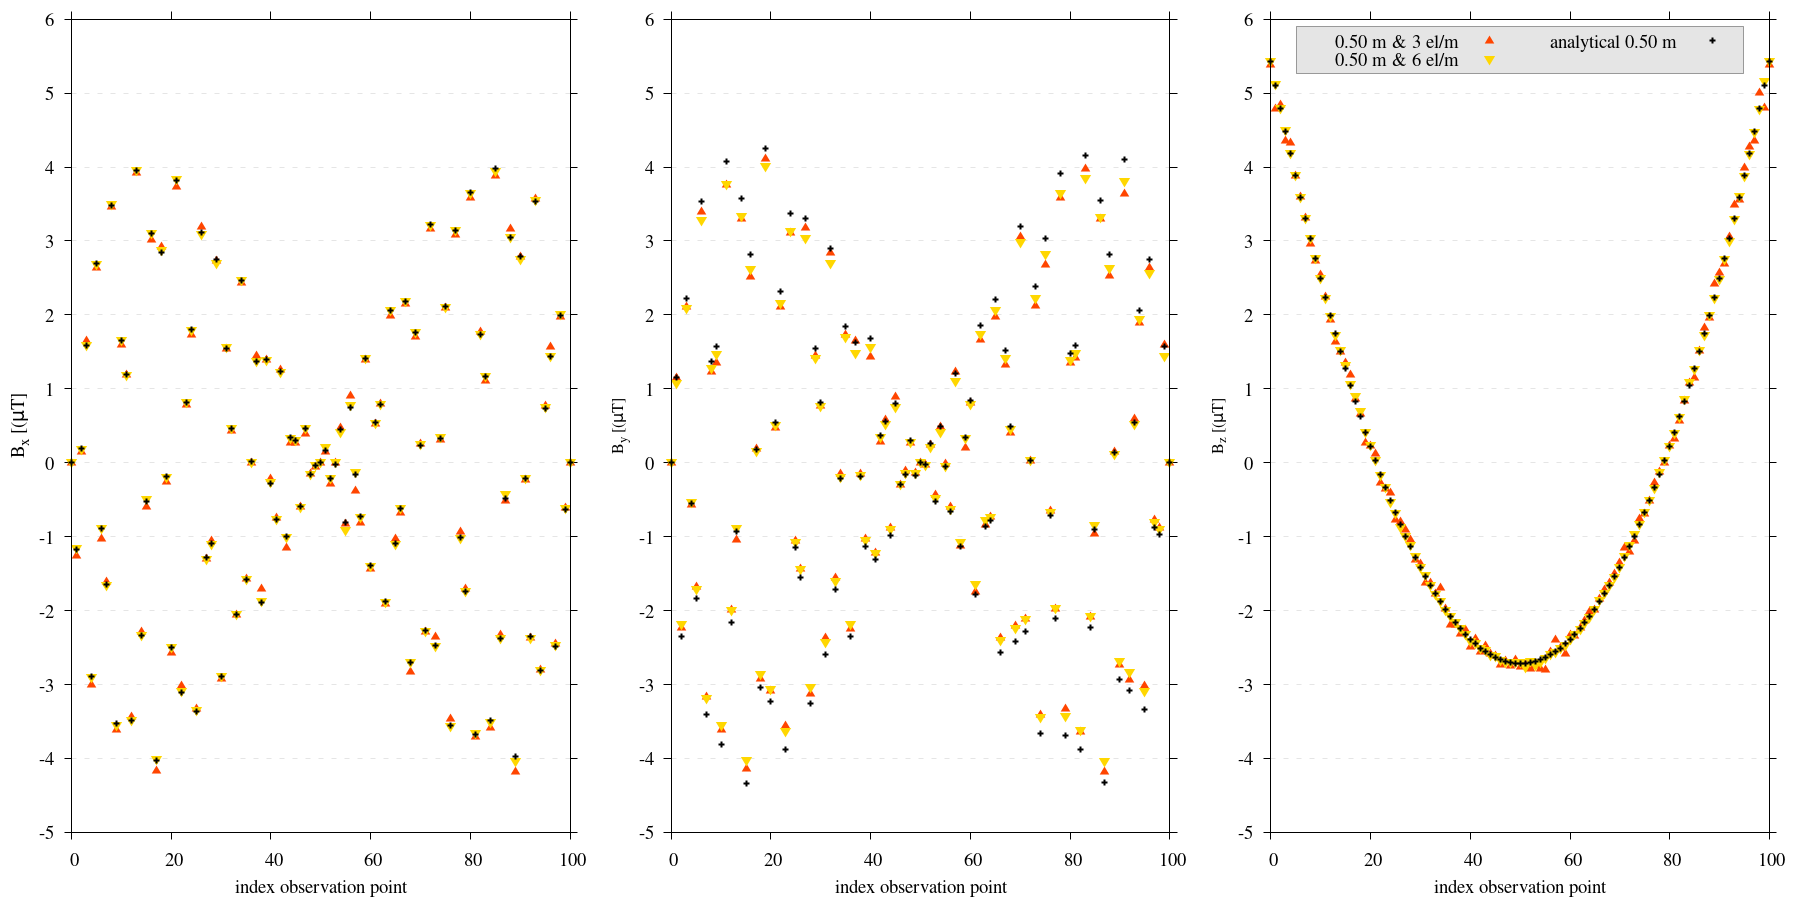
\includegraphics[width=1\columnwidth]{Afbeeldingen2/Benchmarks/B3sphere_mp_05.png}
    \caption{Difference between analytical solution and computed values for 100 difference computation points at either 0.25 or 0.5m above the surface of a sphere with a resolution of either 3 or 6 el/m. Numbering of the computation points start at the top of the sphere and circle down in a counterclockwise fashion.  }
    \label{fig:sphere_bench}
\end{figure} 

